\chapter{Parameterliste} \label{ch:Parameterliste}
\begin{table*}[ht]
	\centering
		\begin{tabular}{|cccc|}
		\hline
		\textbf{Parameter} & \textbf{Variable} & \textbf{Wert} & \textbf{Quelle} \\ \hline
		\multicolumn{1}{|c}{Masse Ball} & \multicolumn{1}{c} {$m_{S}$} &  \multicolumn{1}{c} {0,3280 kg} & \multicolumn{1}{c|} {Gemessen}  \\ \hline
		\multicolumn{1}{|c}{Masse Motor} & \multicolumn{1}{c} {$m_{M}$} &  \multicolumn{1}{c} {0,0820 kg} & \multicolumn{1}{c|} {Datenblatt}  \\ \hline
		\multicolumn{1}{|c}{Masse omnidirektionales Rad} & \multicolumn{1}{c} {$m_{OW}$} &  \multicolumn{1}{c} {0.0520 kg} & \multicolumn{1}{c|} {Gemessen}  \\ \hline
		\multicolumn{1}{|c}{Masse virtuelles Rad} & \multicolumn{1}{c} {$m_{W}$} &  \multicolumn{1}{c} {0,4020 kg} & \multicolumn{1}{c|} {Gemessen}  \\ \hline
		\multicolumn{1}{|c}{\begin{tabular}[c]{@{}c@{}}Masse Roboterk�rper\\ (mit Motoren/R�der)\end{tabular}}  & \multicolumn{1}{c} {$m_{B}$} & \multicolumn{1}{c} {1,603 kg} & \multicolumn{1}{c|} {Gemessen}\\ \hline
		\multicolumn{1}{|c}{\begin{tabular}[c]{@{}c@{}}Masse Roboterk�rper\\ (ohne Motoren/R�der)\end{tabular}}  & \multicolumn{1}{c} {$m_{B}$} & \multicolumn{1}{c} {1,2010 kg} & \multicolumn{1}{c|} {Gemessen}\\ \hline
		
		\multicolumn{1}{|c}{Radius Ball} & \multicolumn{1}{c} {$r_{S}$} &  \multicolumn{1}{c} {0,0800 m} & \multicolumn{1}{c|} {Datenblatt}  \\ \hline
		\multicolumn{1}{|c}{Radius virtuelles Rad} & \multicolumn{1}{c} {$r_{W}$} &  \multicolumn{1}{c} {0,0300 m} & \multicolumn{1}{c|} {Datenblatt}  \\ \hline
		\multicolumn{1}{|c}{Radius K�rper} & \multicolumn{1}{c} {$r_{B}$} &  \multicolumn{1}{c} {0,0703 m} & \multicolumn{1}{c|} {Gemessen}  \\ \hline
		\multicolumn{1}{|c}{H�he Massenschwerpunkt} & \multicolumn{1}{c} {$l$} &  \multicolumn{1}{c} {0.236 m} & \multicolumn{1}{c|} {SolidEdge}  \\ \hline
		\multicolumn{1}{|c}{H�he K�rper} & \multicolumn{1}{c} {$h$} &  \multicolumn{1}{c} {0.366 m} & \multicolumn{1}{c|} {SolidEdge}  \\ \hline
		
		
		\multicolumn{1}{|c}{Tr�gheitsmoment Ball} & \multicolumn{1}{c} {$I_{S}$} &  \multicolumn{1}{c} {0,0013 $kgm^{2}$} & \multicolumn{1}{c|} {Berechnet}  \\ \hline
		\multicolumn{1}{|c}{Tr�gheitsmoment Rotor} & \multicolumn{1}{c} {$I_{M}$} &  \multicolumn{1}{c} {3.8e-8 $kgm^{2}$} & \multicolumn{1}{c|} {Datenblatt}  \\ \hline
		\multicolumn{1}{|c}{Tr�gheitsmoment omnidirektionales Rad} & \multicolumn{1}{c} {$I_{OW}$} &  \multicolumn{1}{c} {2,34e-5 $kgm^{2}$} & \multicolumn{1}{c|} {Berechnet}  \\ \hline
		
		\multicolumn{1}{|c}{\begin{tabular}[c]{@{}c@{}}Tr�gheitsmoment der virtuellen R�der\\ ($yz$- und $xz$-Ebene)\end{tabular}}  & \multicolumn{1}{c} {$I_{W,yz, xz}$} & \multicolumn{1}{c} {0.00357 $kgm^{2}$} & \multicolumn{1}{c|} {Berechnet}\\ \hline
		
		\multicolumn{1}{|c}{\begin{tabular}[c]{@{}c@{}}Tr�gheitsmoment virtuelles Rad\\ ($xy$-Ebene)\end{tabular}}  & \multicolumn{1}{c} {$I_{W,xy}$} & \multicolumn{1}{c} {0.0143 $kgm^{2}$} & \multicolumn{1}{c|} {Berechnet}\\ \hline
		
		\multicolumn{1}{|c}{\begin{tabular}[c]{@{}c@{}}Tr�gheitsmoment K�rper\\ ($yz$-Ebene)\end{tabular}}  & \multicolumn{1}{c} {$I_{B,yz}$} & \multicolumn{1}{c} {0.0880 $kgm^{2}$} & \multicolumn{1}{c|} {SolidEdge}\\ \hline
		\multicolumn{1}{|c}{\begin{tabular}[c]{@{}c@{}}Tr�gheitsmoment K�rper\\ ($xz$-Ebene)\end{tabular}}  & \multicolumn{1}{c} {$I_{B,xz}$} & \multicolumn{1}{c} {0.0880 $kgm^{2}$} & \multicolumn{1}{c|} {SolidEdge}\\ \hline
		\multicolumn{1}{|c}{\begin{tabular}[c]{@{}c@{}}Tr�gheitsmoment K�rper\\ ($xy$-Ebene)\end{tabular}}  & \multicolumn{1}{c} {$I_{B,xy}$} & \multicolumn{1}{c} {0.0070 $kgm^{2}$} & \multicolumn{1}{c|} {SolidEdge}\\ \hline
		
		\multicolumn{1}{|c}{�bersetzungsverh�ltnis} & \multicolumn{1}{c} {$i$} &  \multicolumn{1}{c} {353,5} & \multicolumn{1}{c|} {Datenblatt}  \\ \hline
		\multicolumn{1}{|c}{Erdbeschleunigung} & \multicolumn{1}{c} {$g$} &  \multicolumn{1}{c} {9,81 $\frac{m}{s^{2}}$} & \multicolumn{1}{c|} {Datenblatt}  \\ \hline
		\end{tabular}
\end{table*}
\chapter{ROS-Graph Simulation} \label{fig:rosgraph}
\begin{figure}[htbp]%
	{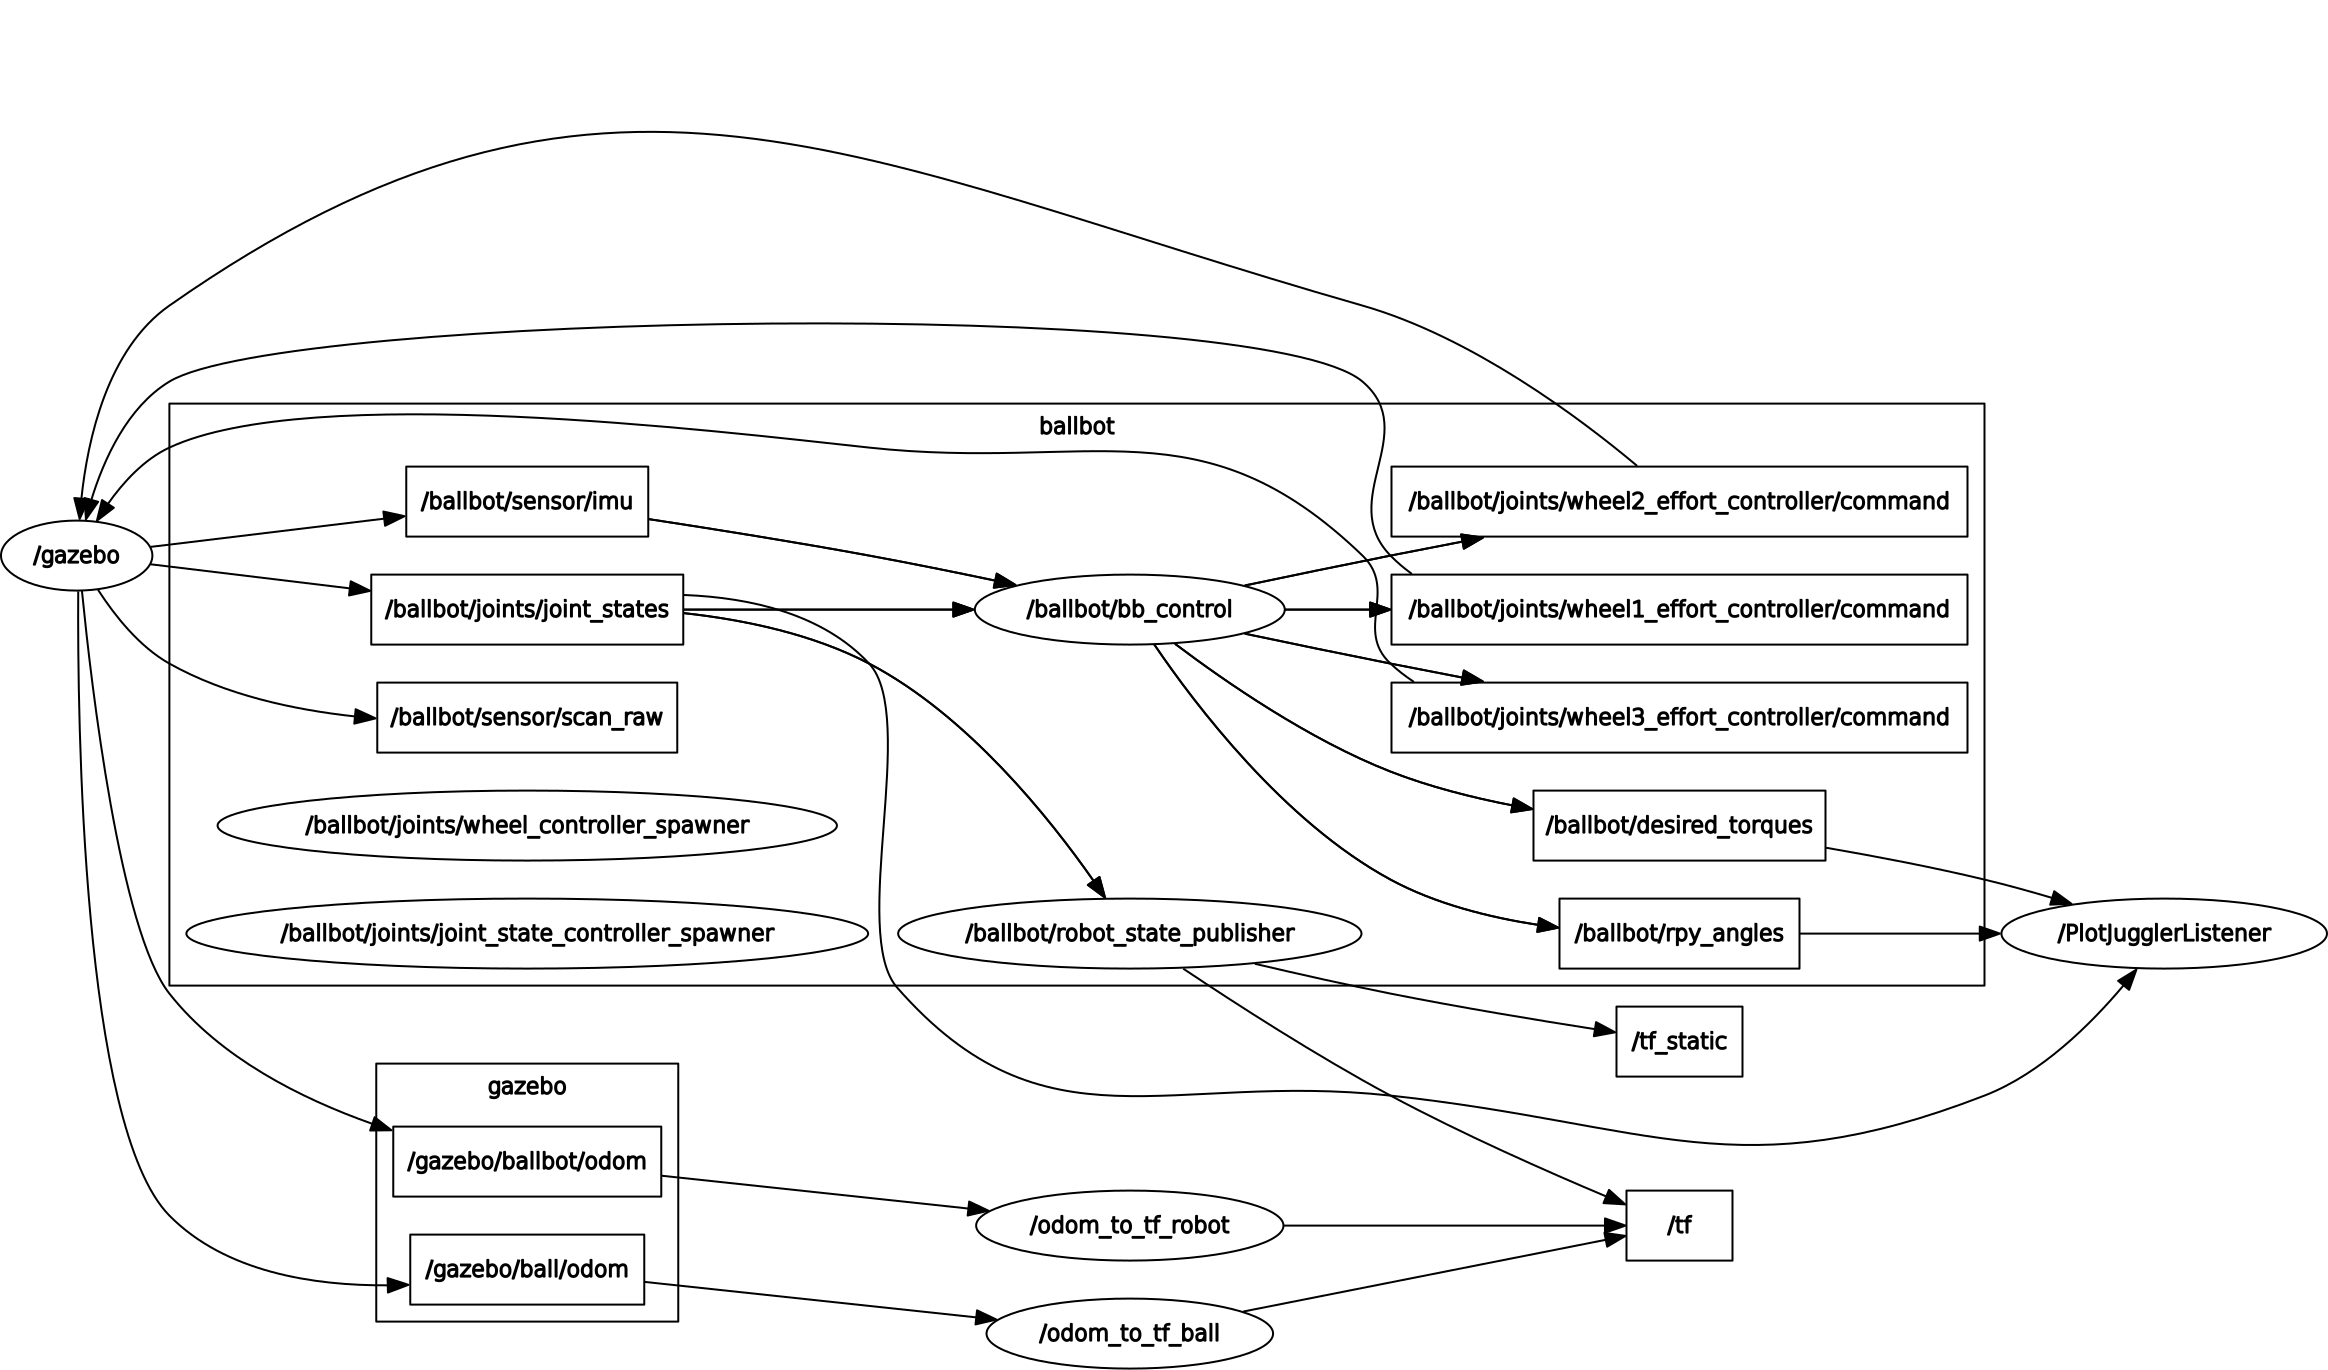
\includegraphics[scale=0.25, angle=90]{./Bilder/Markus/rosgraph.png} }
	\caption{�bersicht aller Teilprogramme(Nodes) und deren Topics, die beim Starten der Simulation aktiv sind und Nachrichten austauschen. Hierbei sind die Nodes mit Ellipsen und die Topics mit Rechtecken gekennzeichnet. Das Bild wurde mit dem ROS Programm rqt\_graph erstellt.}
\end{figure}

\chapter{Simulink Simulationsaufbau} \label{ch:gesamtbild}
\begin{figure}[htbp]%
	{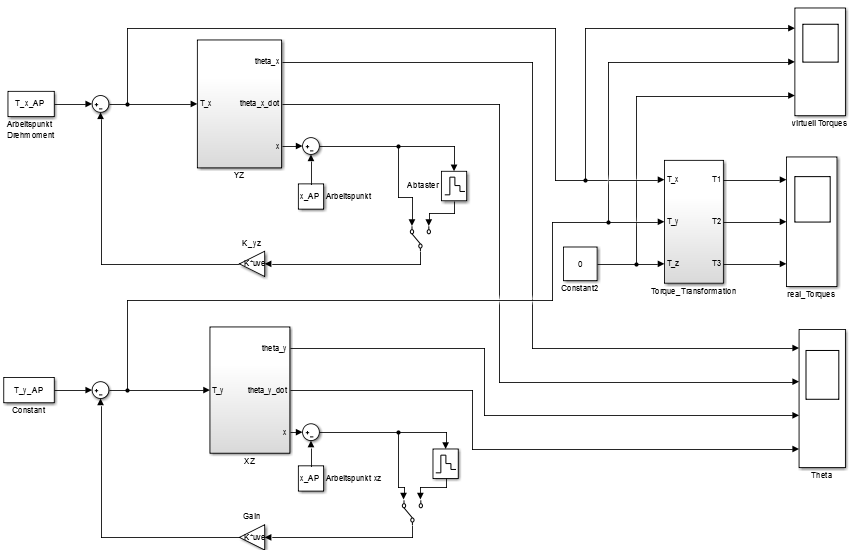
\includegraphics[scale=0.8, angle=90]{./Bilder/Florian/Komplett_System_MATLAB_SIMULINK.PNG} }
	\caption{�bersicht des Simulink Simulationsaufbaus}
\end{figure}
